%-------------------------------------------------------------------------------
% TEMPLATE FOR UCL MSc ECONOMICS THESES
% (c) Elliott Christensen, 2023

% This is a template for a MSc Thesis document based upon a template uploaded by Sofia Feist, 2020. 

% Modified for personal and academic use by Danish bin Abdul Fata (danish.abdulfata.21@ucl.ac.uk).
%------------------------------------------------------------------------------- 


% ------------------ DOCUMENT SETUP ------------------ 
% The document class defines the document type (article) and sets the font size (12pt)
\documentclass[12pt]{article}

% Your name and EXAM CODE
\newcommand{\examcode}{QWJF7}
\author{Dan}

% Inputs the Document Packages
\input{Packages}
% Adds glossary page for acronyms through the glossaries package

\makeglossaries

\newacronym{lcz}{LCZ}{Local Climate Zone}

\newacronym{ucl}{UCL}{Urban Canopy Layer}

\newacronym{ubl}{UBL}{Urban Boundary Layer}

\newacronym{suews}{SUEWS}{Surface Urban Energy and Water Balance Scheme}

\newacronym{supy}{SuPy}{SUEWS as a Python package}

\newacronym{tempair}{T_a}{Air temperature at 2m above surface}

\newacronym{uhi}{UHI}{Urban Heat Island}

\newacronym{gkl}{GKL}{Greater Kuala Lumpur}

\newacronym{enso}{ENSO}{El Niño-Southern Oscillation}

\newacronym{lsm}{LSM}{Land Surface Model}

\newacronym{gee}{GEE}{Google Earth Engine}

\newacronym{eo}{EO}{Earth Observation}

\newacronym{mc}{MC}{Maritime Continent}


% Controls how many subsections the document can take
%  and how many of those will get put into the contents pages.
%\setcounter{secnumdepth}{3}
% \setcounter{tocdepth}{2}

\hypersetup{
  colorlinks,
  citecolor=black,
  linkcolor=black,
  urlcolor=blue}

% Line Spacing
\setstretch{1.5}

% The folder path where the images will be uploaded
\graphicspath{ {./Image/} } 

% Places a dot after Chapter/Section/Subsection number in Table of Contents
% \renewcommand{\cftchapaftersnum}{.}
\renewcommand{\cftsecaftersnum}{.}
\renewcommand{\cftsubsecaftersnum}{}

%  Customize Dot spacing in Table of Contents/List of Figures/Tables
\renewcommand{\cftdotsep}{0.3}

% Numeration Type for Chapters and Sections (Roman I, II, II / Arabic 1, 2, 3)
% \renewcommand\thechapter{\Roman{chapter}}
\renewcommand\thesection{\arabic{section}}

% Line Break Properties
\tolerance=1
\emergencystretch=\maxdimen
\hyphenpenalty=10000
\hbadness=10000

% Formatting Table of Contents/Lists titles
\renewcommand{\contentsname}{\normalfont\bfseries\LARGE{CONTENTS}}
\renewcommand{\listfigurename}{\normalfont\bfseries\LARGE{LIST OF FIGURES}}
\renewcommand{\listtablename}{\normalfont\bfseries\LARGE{LIST OF TABLES}}


% Title Formatting customization

\titleformat{\chapter}{\bfseries\LARGE}{\thechapter.}{1em}{\MakeUppercase}
\titlespacing*{\chapter} {0pt} {0pt} {0pt} % left, before, after

\titleformat{\section}{\bfseries\Large}{\thesection.}{1em}{\MakeUppercase}
\titlespacing*{\section} {0pt} {0pt} {0pt}

\titleformat{\subsection}{\bfseries\normalsize}{\thesubsection}{1em}{}
\titlespacing*{\subsection} {0pt} {10pt} {10pt}

\titleformat{\subsubsection}{\itseries}{}{1em}{}
\titlespacing*{\subsubsection} {0pt} {10pt} {10pt}

\titleformat{\paragraph}{\normalsize}{}{}{}
% HEADER AND FOOTER
\pagestyle{fancy}  % Set Page Style (Header and Footer Style)
\fancyhf{}  % Clears the header and footer (from the default info)


% Add a horizontal line by removing the % sign before the renewcommand (or vice versa): 
\renewcommand{\headrulewidth}{0.1pt}

% Header
%\fancyhead[L]{\bfseries{UCL Geography 2024-25}}
\fancyhead[L]{\nouppercase{\leftmark}}
\fancyhead[C]{\bfseries{\examcode}}
\fancyhead[R]{GEOG0037}

% Footer
\fancyfoot[C]{\thepage} % Page Number


% Only footer page style (removes header when specified)
\fancypagestyle{only_footer}[fancy]{
\fancyhead{}%
\renewcommand{\headrulewidth{0pt}}% overrides previously defined line width when style is applied
}

% Change figure numbering per section
\numberwithin{figure}{section}
\numberwithin{table}{section}

% Defining custom lists
\newlist{declarationterms}{enumerate}{1}

% Defining "comment" command for multi-line comment blocks.
\newcommand{\mycomment}[1]{}

%  -------------------------------------------------
%  --------- The document starts from here --------- 
%  -------------------------------------------------

\begin{document}

% ------------------  TITLE PAGE -------------------
% ASK FOR UPDATED COVERSHEET!!!
\begin{titlepage}
\begin{center}
    % UCL IMAGE
    \vspace*{-3.5cm}
    % Choose colour from the Image Folder: More can be found here: https://imagestore.ucl.ac.uk/imagestore/start/ucl-banners/For%20PRINT/UNCOATED/DL%20PORTRAIT?fc=browse&column=5
    \makebox[\textwidth]{
\includegraphics[width=211mm]{Image/ucl-banner-dl-port-darkblue-u.eps}}
    \vfill % Elastic empty space filler
    
    % Title
    {\LARGE\textbf{Modelling the spatio-temporal urban heat island effect of a tropical city:\\}}
    
    % #Modelling the spatiotemporal variation of the Urban Heat Island of Greater Kuala Lumpur
    % Modelling the spatiotemporal urban heat island effect of Greater Kuala Lumpur: a case of the lightweight land surface model Surface Urban Energy and Water Balance Scheme (SUEWS)
    
    % Subtitle
    {\LARGE\textbf{The case of Greater Kuala Lumpur\\}}

    \vspace{0.8cm}
    by\\
    \vspace{0.8cm}

    % Author
    {\LARGE\textbf{\examcode\\}}
    % Date
    \vspace{1.5cm}
    {\Large\textbf{Academic Year 2024-25}}

    \vfill

    \textbf{\setstretch{2.0} 
    Dissertation Supervisor: Dr Chris Brierley, UCL Geography\\
    \vspace{1cm}
    GEOG0037 45-credit Dissertation written in contribution to the\\
    Degree of Bachelor of Science in Geography\\
    \vspace{1cm}
    Department of Geography\\
    University College London\\}

    \vspace{2cm}
\end{center}
\end{titlepage}

% -------------------  DECLARATION ---------------------

\clearpage

\thispagestyle{empty} % removes header and footer
\addtocounter{page}{-1} % subtracts page number by -1, ie. ignores this page when counting

\begin{center}
    % UCL IMAGE
    \vspace*{-3.5cm}
    \makebox[\textwidth]{
\includegraphics[width=211mm]{Image/ucl-banner-dl-port-darkblue-u.eps}} % UCL banner image directory
    \vfill
        {
        \setstretch{3.0} % somehow fixes unbalanced spacing issue between title/subtitle, banner and footnote. 
            {\LARGE\textbf{DEPARTMENT OF GEOGRAPHY}}\\
            {\Large\textbf{BSc Geography}}
        }
\end{center}

\noindent\footnotesize{%
Please complete the following declaration and include this form after the title sheet of your dissertation.
}

\noindent\normalsize\textbf{%
    I, \examcode \\
    hereby declare:}
\begin{declarationterms}
    \footnotesize
    \setstretch{1.5}
    \setlength{\itemsep}{1pt}
        \item[(a)] that this dissertation is my own original work and that the exact source of any material (ideas, information, figures or text) derived or quoted from the published or unpublished work of other persons has been cited according to the required conventions 
        \item[(b)] that I have read the UCL Academic Integrity policy on plagiarism, self-plagiarism, collusion, falsification and contract cheating
        \item[(c)] that the dissertation has been prepared specially for the BA/BSc in Geography of UCL (University College London);
        \item[(d)] that the dissertation does not contain any material previously submitted to the examiners of this or any other University, or any material previously submitted for any other examination. 
\end{declarationterms}
\noindent\textbf{%
Number of words: \\
Signed: \examcode\\
Date: \today 
}

\vfill
{\noindent\small
I acknowledge the use of Artificial Intelligence (AI)}

{\noindent\footnotesize
[insert AI system(s) with link, and number of iterations where appropriate] to [please, provide a detailed description of no more than 250 words about how you used AI]} I used Chat-GPT to help explore options in structuring and visualizing my modelled data. It also helped creating a solution with data misalignment but lead to further problems down the line that I had to troubleshoot and fix.

\vfill

{\setstretch{1.0}\noindent\scriptsize%
Please note that the Department of Geography makes dissertations available online for consultation by other students and staff. They cannot be downloaded. If you wish your dissertation to be excluded from those made available for others to view, please send an email to the relevant dissertation convenor, with a copy to Nick Mann.

\noindent 
For further details about how UCL processes your personal data, please see the \href{https://www.ucl.ac.uk/legal-services/privacy/ucl-student-privacy}{UCL Student Privacy Notice.}
\par}
 % section files are numbered so that Overleaf sorts them chronologically

% ------------------  TABLE OF CONTENTS --------------------
\newpage
\tableofcontents 
\thispagestyle{only_footer}

% ----------------------  ABSTRACT AND ACKNOLEDGEMENTS -----------------------

\newpage
\thispagestyle{only_footer}

% Abstract Page

\section*{\normalfont\bfseries\LARGE{{Abstract}}} % the Asterix (*) indicates that this section will be added to the table of contents but no number will be present beside it.
\addcontentsline{toc}{section}{Abstract}

% Short intro

Urban heat studies often focus on either the city-scale or small street-scale case studies of the \Gls{uhi}, with a demonstrable lack in synthesizing at the medium district or local level. With calls to understand the socially contentious and uneven effects of urban planning, this study provides a potential new method of analysis through running an urban land surface model, \Gls{suews}, to analyze the geospatial unevenness of \Gls{uhi} in the tropical urban agglomeration of Greater Kuala Lumpur. 

% The urban land surface model, \Gls{suews} through python (\Gls{supy}) is run utilizing newly updated and open-source datasets, to simulate near-surface climactic conditions in Greater Kuala Lumpur.


% Methodology






% FIndings


\textbf{Keywords:} Urban Climate, Urban Heat Island, Land Surface Model, Urban Planning, Open Source


% Acknowlegments Page

\clearpage
\thispagestyle{only_footer}
\section*{\normalfont\bfseries\LARGE{{Acknowledgements}}}
\addcontentsline{toc}{section}{Acknowledgements}

% Supervisor: Dr Chris Brierley.
% Dr Ting Sun (RDR)     Technical Supervisor: Dr Ting Sun, UCL Risk and Disaster Reduction\\

Others in UCL Geography that I would like to mention for their patience, empathy and guidance in navigating this challenging and confusing part of my life include Dr Fabien Cante, Dr Ben Page, Professor Jonathan Holmes, Clara Hall and Dr Izzy Bishop. 

\noindent I also deeply value and respect my parents, Abdul Fata Abd Aziz, "Ayah", and Maheran binti Ajis, "Mama", for their continual sacrifices and unconditional support throughout my life in spite of our disagreements and apprehensions. This also extends to my siblings, and especially Fatin Abdul Fata, "Kak Sya", whose continuous contact and help in London I could never repay. 

\noindent Special regards are additionally given to my friends: Azrul Azim Azlan, Kritsada Kaewinta, Mohamed Suliman, Muhammad Moahad Saqib, Nimallan Elangovan and Nsikan Nsikan Umoh for the unceasing and ongoing support throughout difficult periods in my degree.

\noindent I would also like to thank the Malaysian Government for covering my tuition fees through their World Top University Education Loan programme under Majlis Amanah Rakyat (MARA). I am very grateful to have been given the opportunity to study in London.

%
 % Acknoledgements also in 3.abstract. 


% -------------------  LIST OF FIGURES --------------------

\newpage 
%{\let\oldnumberline\numberline       % Uncomment to add the word 'Figure' to figure number in List of Figures
%\renewcommand{\numberline}{\figurename~\oldnumberline}  
\listoffigures%}
\addcontentsline{toc}{section}{List of Figures} % Add List of figures into contents without any numeration 
\thispagestyle{only_footer}

% -------------------  LIST OF TABLES ---------------------

\newpage

\listoftables 
\addcontentsline{toc}{section}{List of Tables} % Add List of tables into contents without any numeration 
\thispagestyle{only_footer}

% -------------------  LIST OF ABBREVIATIONS --------------------
\newpage
\printglossary[title={\normalfont\bfseries\LARGE{LIST OF ABBREVIATIONS}}, toctitle=List of Abbreviations, type=\acronymtype, nonumberlist]
\thispagestyle{only_footer}

% -------------------  Introduction and Literature Review ---------------------

\newpage
\section{Introduction}

% The goal is to not write a passive "policy paper" like the UN, but to utilize EO data and climate modelling as means to guide the poltically informed "conversations" in the dissertation.

\subsection{The Urban Climate}

% Synthesis and summary of social science and science based literature of the urban climate
    % scientific explanations that give way to social-historical results
In the start of \textit{Urban Climates} by urban climatologists \textcite{urban_climates}, the city was described as a "wide array of surface elements of very different sizes and compositions, [with] the vast majority of them [] alien to the natural landscape and include pulses of energy, water, gases and particles \textbf{controlled by people} rather than geophysical activity"(p. xix, author emphasis). This is the crux of understanding the urban climate, whereby the built environment is inherently artificial, in which it's processes are clearly anthropogenic, and where studies must bridge this gap, recognizing that research of the urban environment is thus primarily a study of human processes first and foremost. The traditional division between the "natural" and "social" sciences, and within geography as "physical" and "human" falls apart in the city. This dissertation serves as an exploration of this interdisciplinarity, critically utilizing climate modelling as means of understanding the geospatial inequalities of the \Gls{uhi} in Greater Kuala Lumpur.  %/cite. Page 55 un_2018_wup, 60.4% urbanpop, 27.8% in city >1mill

The world is facing a multitude of crises, environmental, social and economic, that are especially embodied in the urban city. The \textcite{un_2018_wup} estimates that 60\% of the world population, consisting of 5.2 billion people, will be living in urban areas by 2030 with nearly half living in metropolitan areas of greater than a million people. The Global South in particular is facing unprecedented and rapid urbanization, whereby cities like Karachi, Jakarta and Dar es Salaam will overtake well-known Northern agglomerations like New York, Paris and London, with more than 100 settlements having a population of greater than 5 million by 2030. These urban agglomerations have grown to such an extent to have noticeable effects on their regional climates, with numerous studies having established that urban environments are prone to rising surface and urban temperatures, alterations of precipitation patterns and intensity at both a sub-daily and seasonal scales, the destruction of natural ecosystems, and a complicated interaction of this large urban ecosystem with it's peri-urban 'semi-natural' surroundings. 

Understanding the biophysical and social processes that dictate and govern the living conditions for a majority of mankind becomes not only a matter of scientific curiosity but a social necessity to equip those most affected with the knowledge and tools to rewrite their own circumstances (\cite{crit_physicalgeo}). Echoing this sentiment, there is an urgent need to carry forward the goal of 'common but differentiated responsibilities and respective capabilities' in response to anthropogenic climate change (\cite{paris_agreement}). However, in practical terms, there is still a consistent "data gap" between the Global North and South, which means there is considerable difficulty for research to be equitable and consistently accurate between different regions. In addition to this data gap, Southern nations face additional challenges in adapting and responding effectively to the rapid growth of their cities, which often coincide with notions of economic progress and development (\cite{urban_resilience}). Socioeconomic and political factors continuously limit the ability for governments and other institutions to setup and gather data in many of these "informal" urban growths, and scholarship bias to Northern urban environments leads to a lack of established literature and relevant procedures to design comparable and reproducible studies of Southern urban climates.


The call for a critical physical geography by \textcite{crit_physicalgeo} is especially relevant for urban climate research, where the resulting environmental conditions and research itself is a direct result of political-economic decision-making. Initiatives for utilizing academically rigorous, neutral and globally available datasets, with open-source and replicable methodology, is prudent in bridging this gap while enabling accessible 'citizen science'.

This dissertation utilizes an open-source and standardized methodology of simulating the the urban climate of Greater Kuala Lumpur to further inform discussions regarding the unequal geospatial effects of the \Gls{uhi} and their potential social effects in the Greater Kuala Lumpur urban form and function. 



% expounding general example of city environments and their impacts on climactic conditions
 
% sociopolitical risks, urban planning,



\subsection{Urban Climate Modelling}
% Urban Climate Science? The field of Urban Climate?
% The scientific (ie. conceptual) basis of Urban Climate

In the era of big data, and a proliferation of Earth System Science modelling through global \Gls{eo} data, this full head-on engagement with derived information without on the ground measurements  

There has been a lack of synthesizing \Gls{eo} datasets in informing decision-making at a sub-national level due to the complexity of downsizing the data to a smaller level capable of accurately portraying 

% biophysical factors affecting the urban climate

% rise of computational modelling, development of procedures and related modelling work
Climate modelling over the past couple of decades have seen a revolutionary breakthrough as advanced in technology has made it possible to calculate 

Land Surface Models aim to understand the interactions between the surface and atmospheric layers.
% what is it? what are it's mechanisms? what makes it different?
UBL, UCL

%the role of the urban form

% the meso and micro scale

\subsection{Health impacts of Heat Stress}



\subsection{Current Urban Heat research}
The IPCC AR6 report has confirmed that heat stress remains one of the many challenges faced by growing urban environments

The urban heat island has been an established concept in urban climatology for more than half a century (\cite{oke_1973}), primarily due to observed experience and the growth of urban environments. One key way to conceptualize urban heat is through the energy balance at the surface, in which urban environments, having morphometric properties different to that of rural environments, lead to an increase in energy intake and thus air temperature in a city (\cite{urban_energy_balance}). Most research has focused on Northern cities and so understanding the mechanisms of urban heat are still scant in tropical climate regimes where intra-annual temperatures vary less than diurnal ranges. Furthermore, tropical climate regimes face seasonal variations in precipitation which will affect the mentioned urban energy balance equation by introducing varying levels of latent heat flux.

A systemic literature review carried out by \textcite{kim_2021} has found that most urban heat studies can be categorized into two main methodologies, namely experimental or empirical. Due to the difficulty of getting accurate and widespread meteorological data for many of the sites concerned, many research papers that utilize experimental designs
The \Gls{uhi} phenomenon has been noted since xy 

Many papers utilize numerical simultions such as that of the WRF model

As many urban climatologists have noted, \Gls{uhi} suffers from a lack of standardization of categories and definitions. In this paper, the focus will be on the Urban Heat Island at 2m air temperature, following the conventional standards for urban heat island studies,



The dissertation will fall under the experimental study, with specific focus on se

(insert UHII equation)
Urban Heat Island Intensity 



% urban heat island effect, and associated literature

% definitions
% Use standardized or proposed standardized UHI units and symbols!!! 

% understanding the differences between UHI from surface studies ie. radiative measurements, UHI in the UCL (10-20m dependning on local morpholgoy), UHI in the UBL (<100m). THe study focuses on T2M,

% Ditstinction between surface UHI and etc

% health effects

% Limitations moved to under current heat reserach

A lot of climate modelling not only uses globl big data networks of Earth Observation data, this leads to layers of abstraction t

% local scale (1km and sub 500m) climate modelling, lack of data and high computer usage



\newpage
\section{Site of Study}
    
\subsection{Social and historical background}

\gls{GKL}, also known as Klang Valley (\cite{epu}), is a large urban conurbation in Malaysia consisting of multiple local authorities including that of the capital city of it's name, the Federal Territory of Kuala Lumpur. The city is currently estimated to have a population of nearly 9million, with future projections 


population

brief history, fishing vilalge etc
    % urbanization, expansion
    % urban planning strategies, neoliberal private-led development
    % high rises 

\subsection{Climactic and environmental background}

\Gls{gkl} is located on the confluence of the Klang and Gombak rivers, with an extensive urban sprawl that reaches the coastline at Port Klang. As a result, while not directly at the coast, the city experiences notable coastal influences in it's climate, especially that of land-sea breezes. Additionaly, the Titiawangsa mountain range serves as a great central divider of Peninsular Malaysia, located to the city's northeast. 

%add topograhical map of peninsular Malaysia, with state boundaries and box of site of study
%zoom in figure 

\Gls{gkl} falls under the meteorological \Gls{mc}, in which diurnal patterns remain the focal point and main driver of larger scale climactic processes. 

% add satelite and topographical image of the study area
    % overlay with model area?
% climactic and meteorological background of the Greater Kuala Lumpur
    % the two monsoon seasons
    % rainfall patterns

% Exisitng urban heat studies
% \subsubsection

In the context of Malaysia, most studies still employ global datasets with sparse data resolution without modelled downscaling . Gl

\subsection{Aims and Objectives}

{\textit\large{Main research question}}
- How does local-scale urban morphology affect the spatio-temporal intensity of the urban heat islands in the tropical climate of Greater Kuala Lumpur?

{\textit\large{Aims}}
- To learn and utilize Python for data science
- 
   % - *surface cover fractions: normal = through LCZ, modified = alteration of default cover fraction conversion parameter
   % - *Independent variable: GKL land cover over time*
   % - *Dependent variable: near surface temperature (2m), relative humidity*


- What are the spatial variations of \Gls{uhii}?
    - *Which parts of GKL exhibit largest UHII? Does this pattern hold over time?*

- What are the diurnal and seasonal patterns of the UHII?





% -------------------  Methodology ---------------------

\newpage
\section{Methodology}

% \subsection{The Urban Heat Island}


\subsection{The SUEWS Model}

The study utilizes an open-source \Gls{lsm} known as the Surface and Urban Energy Balance Scheme (\Gls{suews} from now on, see for example \cite{suews} and \cite{suews2}) through it's bundled Python package \Gls{supy} (\cite{supy2024.7.12}), taking in commonly available meteorological data to model the energy and water balance of the urban surface as shown in Figure~\ref{fig:suews_equations}. Coupled with the heat flux is the modelling of water fluxes that forms the second half of the model's calculation of the energy budget. Thus, the model uses an evaporation-interception approach of the urban surface that feeds into the prior energy balance equation under latent heat flux (Figure~\ref{fig:evapotranspiration_interception_model}, \cite{urban_energy_balance} and \cite{evapotranspiration_interception}). The \Gls{lsm} utilizes multiple sub-models to minimize the amount of forcing data needed to run the model (see \cite{suews} for specifics).

\begin{figure}[bh]
    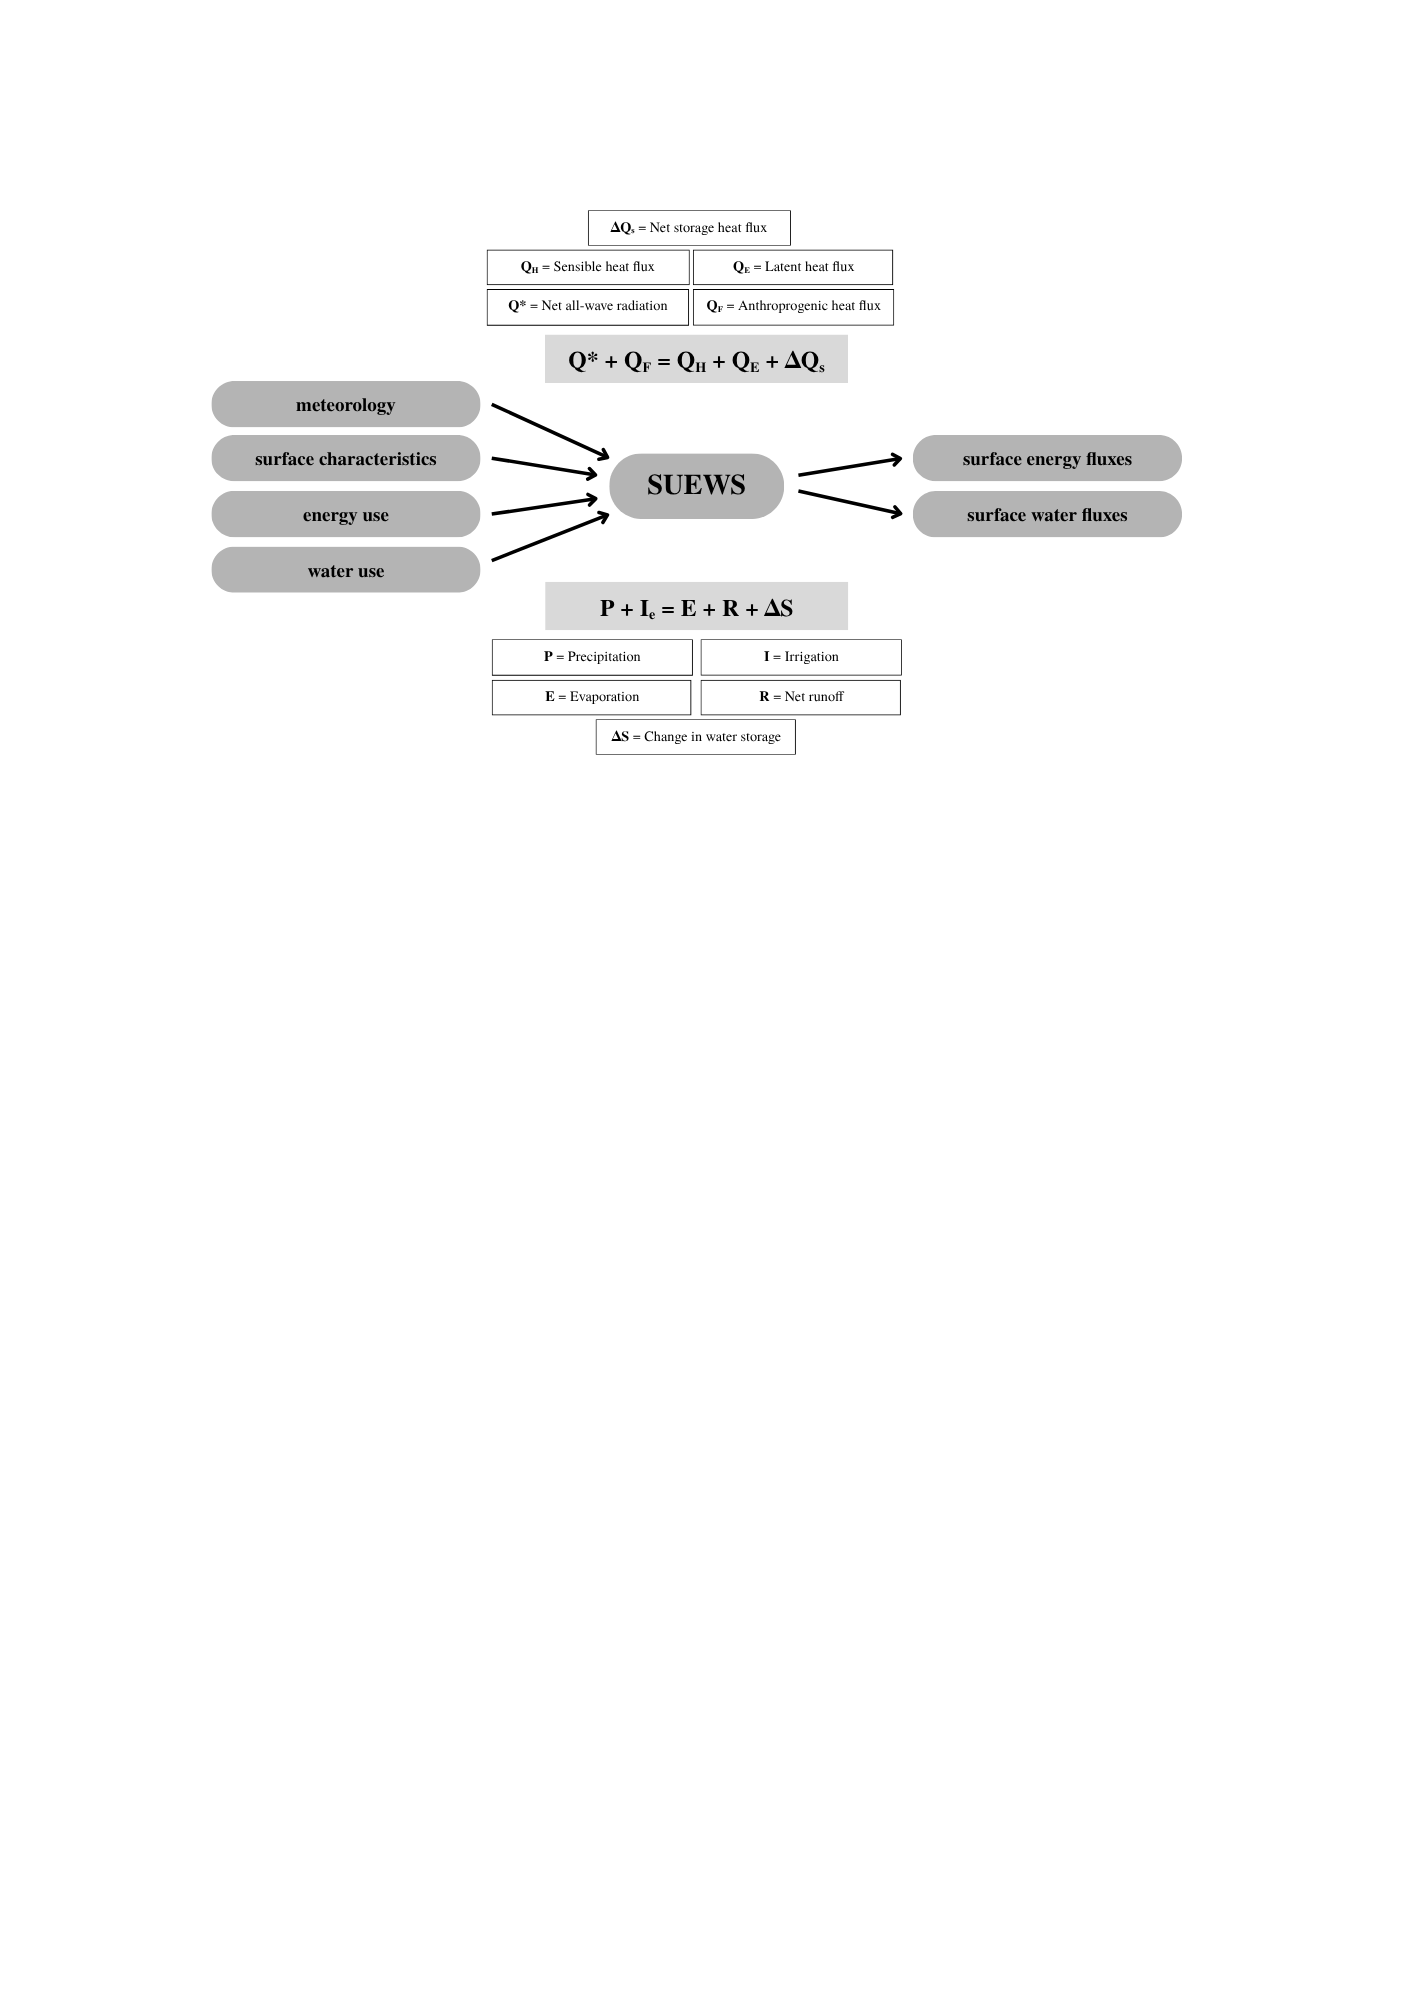
\includegraphics[center, clip, trim = {2cm 17cm 2cm 2cm}]{Image/suews_equations.png}
    \caption{The basic inputs and outputs of SUEWS, adapted from the documentation of \Gls{suews} in \textcite{supy2024.7.12}.}
    \label{fig:suews_equations}
\end{figure}

\begin{figure}[th]
    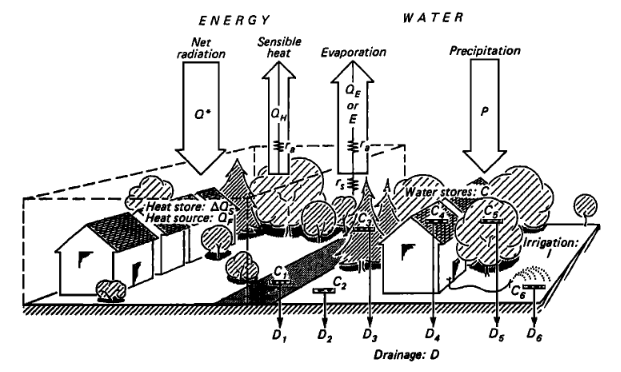
\includegraphics[scale = 0.7, center, clip]{Image/evapotranspiration_interception_model.png}
    \caption{The evapotranspiration model used in SUEWS, taken directly from \textcite[p.1740]{evapotranspiration_interception} where symbols are fully described.}
    \label{fig:evapotranspiration_interception_model}
\end{figure}

Figure~\ref{fig:evapotranspiration_interception_model} showcases the treatment 
single-layer moisture stores 

% 7 different surface cover fractions figure



\subsection{Model Setup}

The \Gls{supy} Global Workflow is a private university GitHub repository by UCL's Department of Disaster and Risk Reduction, where a set of  scripts obtains the necessary input data through the \Gls{gee} API and directly feeds it into \Gls{supy} by simply setting a site's central coordinates. The full process is captured in Figure \ref{fig:process_flowchart}, with the full list of data sources used for the model. \Gls{supy} package version of '2024.7.12.dev' was used for the study (\cite{supy2024.7.12}) with the model running with the default \Gls{supy} sample data for initial soil conditions. The site was run with a spin-up of 2 months to counteract this data unavailability of local soil conditions and to minimize potential errors due to the sensitivity of \Gls{suews} and other \Gls{lsm}s to initial ground and soil conditions (\cite{initial_conditions}). \Gls{supy} was configured to run near the centre of Greater Kuala Lumpur with a total study area of 40km\textsuperscript{2}. Due to computational and data limitations of the \Gls{gee} API, the \Gls{supy} Global LCZ Workflow was ran through multiple instances sequentially to cover the large study area (Figure \ref{fig:process_flowchart}). 2017 forcing in particular was chosen due to a lack of significant weather extremes and to represent a neutral \Gls{enso} state (\cite{mmd_report}). The model takes about 10 hours to complete using the author's personal computer.

% flow chart
\begin{figure}[htb]
    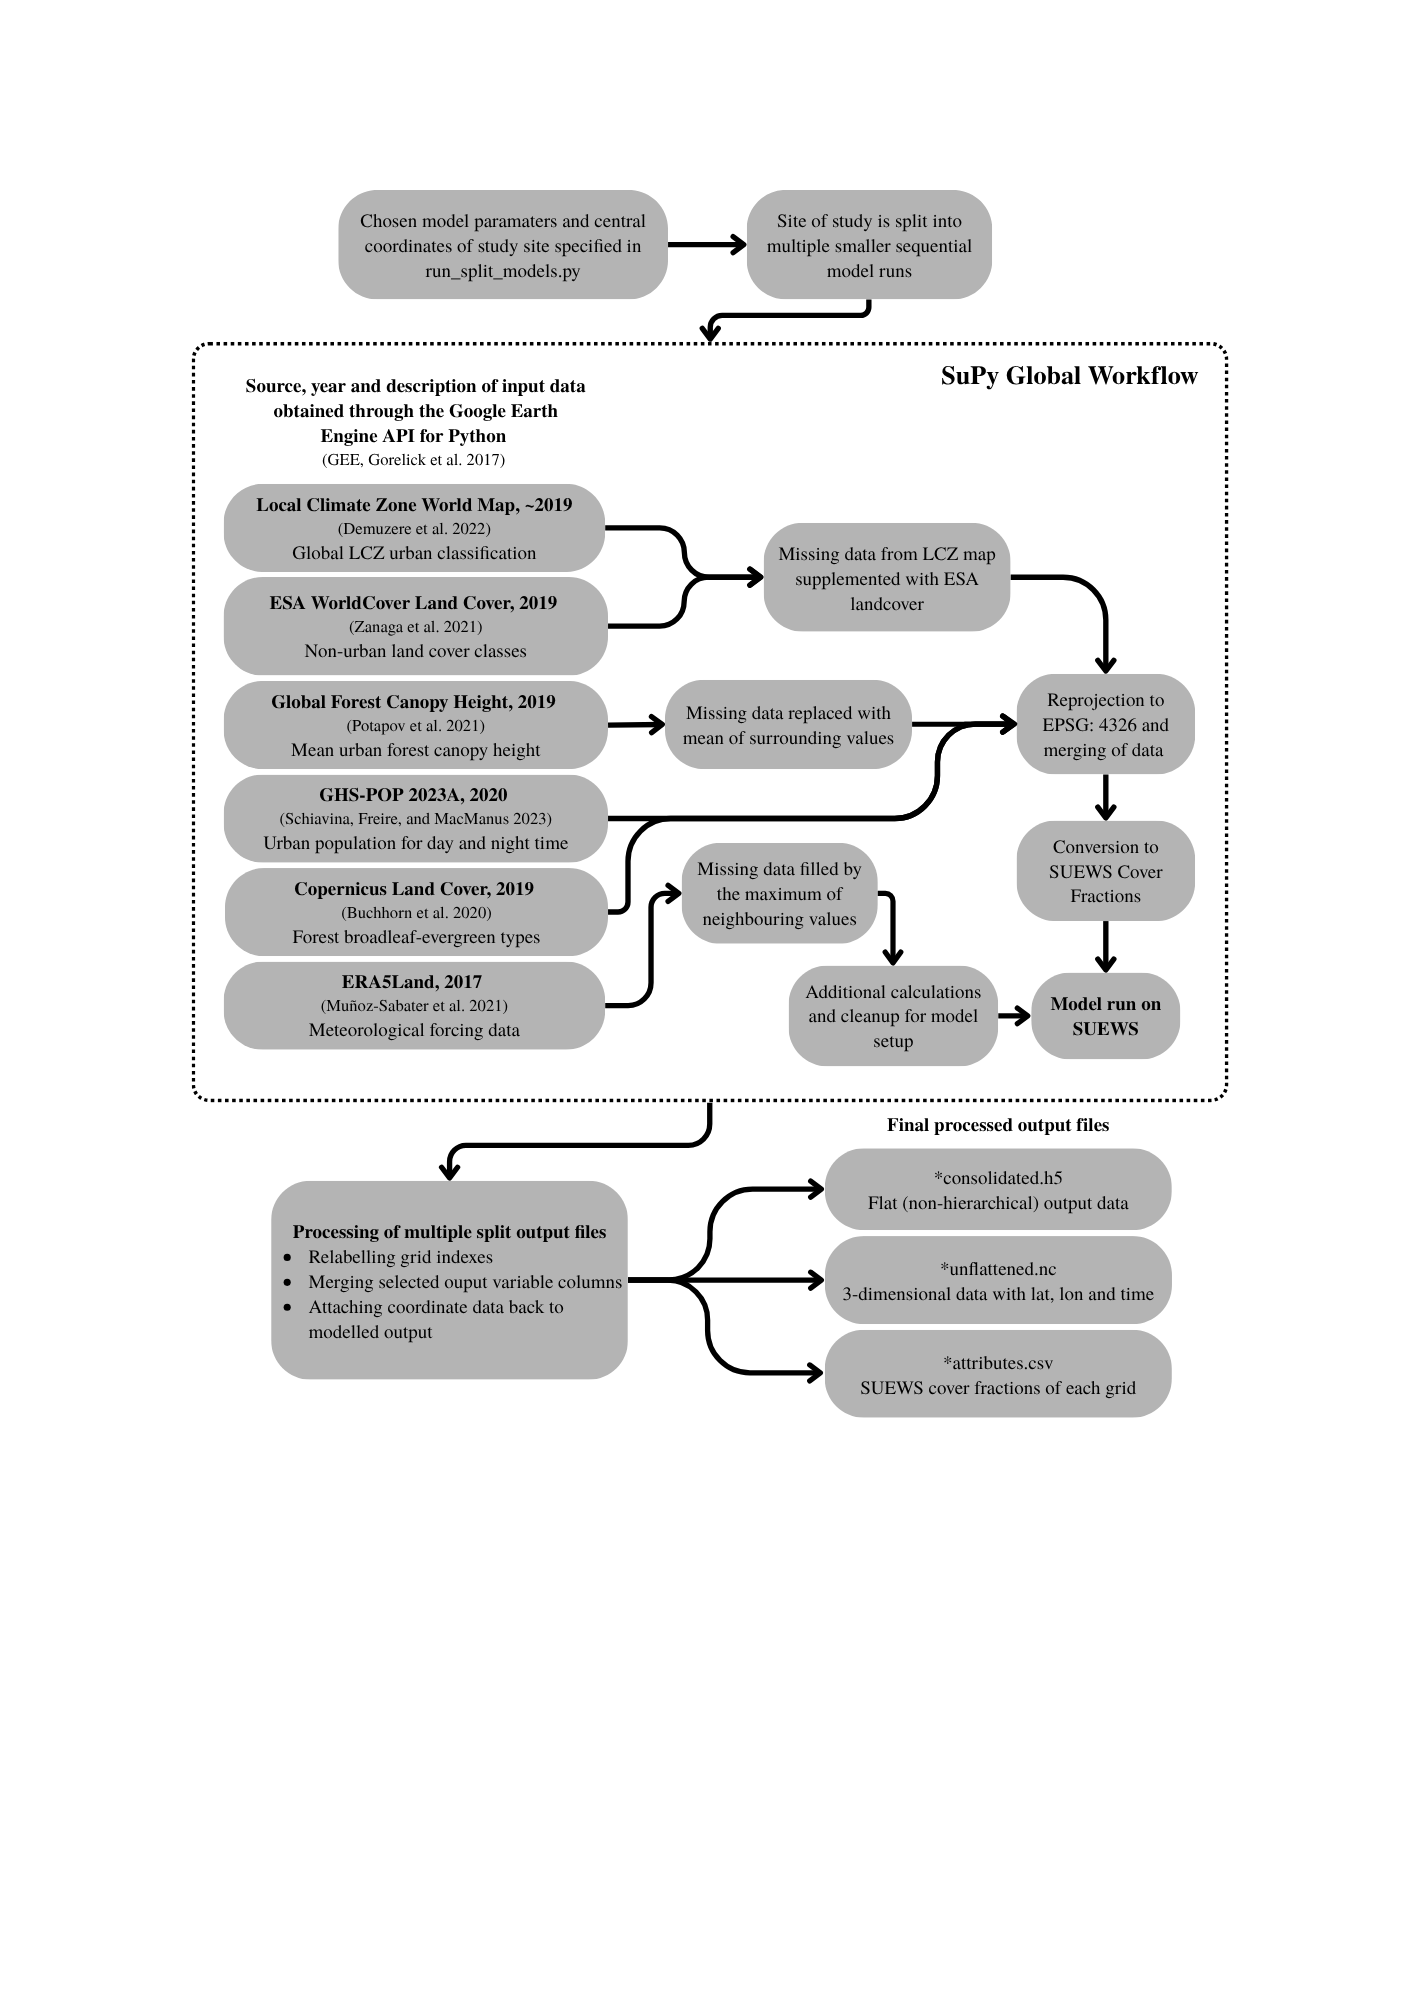
\includegraphics[center, clip, trim = {2cm 5cm 2cm 2cm}]{Image/process_flowchart.png}
    \caption{Flowchart depicting the process of running SUEWS and the \Gls{supy} Global Workflow used for the study, with specific details on data sources and error handling.}
    \label{fig:process_flowchart}
\end{figure}

\subsection{Data Sources}

The workflow relies on a globally available map of \Gls{lcz}, which is an established typology for urban morphology, categorizing urban environments by structure, cover and human activity, resulting in 17 classifications for standardized use in urban heat studies (\cite{lcz}). The Global map of \Gls{lcz}s were derived from a set of human-curated training data that fed into a machine learning classification algorithm of Earth Observation data (\cite{lcz_map}). Land cover information from \textcite{copernicus_lc} was used to identify any missing data which was supplanted through the modal value of surrounding pixels. This \Gls{lcz} map was then fractionated to take into account the model grids being larger than the LCZ map pixels, and then parameterized into author-specified surface cover fractions understandable to \Gls{supy} (Figure \ref{fig:process_flowchart} and see Appendix for tabled parameters). 

Furthermore, \Gls{suews} utilizes population density data from \textcite{popden} to calculate waste heat released through human energy consumption, using a modified approach employed by \textcite{anthropogenic_heat}, where days above and below the baseline temperature of human comfort are termed heating or cooling days. This then provides the model the ability to differentiate the days in terms of energy consumption, thereby providing greater accuracy in estimating energy usage at a finer spatial-temporal scale usually unavailable and difficult to measure directly (\cite{suews}). Figure \ref{} depicts the raw population data and \Gls{lcz}s of the site of study.  The global forest canopy height map by \textcite{forestcanopyheight}) and the ESA WorldCover \textcite{esa_worldcover} are the last two data sources used by the workflow to provide details on the biological components, particularly tree canopy height and the composition of the surface between broadleaf and evergreen forests, which will have a seasonal affect on surface albedo. In the case of \Gls{gkl}, this component is less important as the area is overwhelmingly composed of evergreen forests. 

% LCZ and POPDEN sitemap

\mycomment{
All sourced through the Google Earth Engine API and year of data used and processed through SuPy
    - ERA5Land (2017, author specified), \cite{era5land}
    - GHS-POP 2023A (2020), \cite{popden}
    - LCZ World Map (~2019, multi-year sourced),  \cite{lcz_map}
    - ESA WorldCover 10m v100 Land Cover Fractions (2020), \cite{esa_worldcover} LUC (to identify missing LCZ/Era5Land grtids/pixels and "filling them out"
    - Global Forest Canopy Height (2019), \cite{forestcanopyheight} % Average Height
    - Copernicus Global Land Cover (2019), \cite{copernicus_lc} % for evergreen-broadleaf distinctions
}


\subsection{Suitability}

% previous studies and applicability etc
% add discussion on the role of big data and critically using globally available datasets.
% why SUEWS? alternatives, and current existing papers using the model

The model has been evaluated in the similar tropical urban climate regime of Singapore, using real-world validation data (\cite{demuzere_singapore}). 

\cite{chua_evaluation} 

\subsection{Data Analysis Methods}

% Table of Monsoon dates.

%which noted specific parameterization sensitivities

% add basic UHI equation


% might remove 
% validation and evluation 
        % radiation and heat flux values should look/map reasonable
    
% map making
% The maps were made through a combination of the python package matplotlib and qGIS

% using individual sites as examples

% involving wind speed (10m agl), humidity, and surface temperature variables?

% summary statistics and statistical significance
% statistical significant means




% -------------------  Results and   ---------------------

\newpage
\section{Results}

% all the figures go here frfr

% some values to think about deriving:


% UHI Intensities
    % what time are they the highest
    % in what areas are they the highest
    % seasonality
    % 

% example sites and their socio-political configurations

- current idea: basic T2 seasonal and daily variations and UHII equivalents -> introduce relative humidity and wet bulb tempeature calculations

- final analysis will then be on heat stress and uhii mitigation?


% sort of presentations: 
    % grids with days above certain temprearture thresholds (35C max or 25C min)
    % 

Urban Heat intensities seasonaliity and hourly

Average mean, max and min temps?


% -------------------  Discussion  ---------------------

\newpage
\section{Discussion}

Good workflow for data-sparse regions using global open source datasets.



The LCZ Suews workflow can be used fo rintiial assessments of spatio-temporal spread of urban heat, which can then inform more local and direct studies and methods 

% \subsection{Uncertainties and Limitations} ?

\mycomment{

depending on which scenario I take for calculating the UHI:

1. counterfactual model limitations

2. site-specific comparisons 

}

% potential "circular reasoning"feedback, as ERA5Land data is derived from weather stations measured in urban contexts, even after efforts at removing effects near-surface configurations

% use of EO data presumes accuracy or representative of actual site conditions - find that paper 
    % under the remote sensing module, that phrase the professor used

% accuracy of LCZ Map and it's methodology.

% ïdealized "weather conditions". only 2017 ENSO-netural


% Further research

 Use of \Gls{suews} for modelling the necessary meteorological environment during heat waves and health risks


Utilizing this workflow for multitemporal studies across multiple years through custom LCZ information to model land-use and land-cover changes. 

Utilizing smaller modelled grids for finer details

validation testing?





% -------------------  Conclusion ---------------------

\newpage
\include{8.conclusion}

% -------------------  Auto-critique ---------------------

\newpage
\pagestyle{only_footer} % overrides /pagestyle to only show footer from now on.
\section*{\normalfont\bfseries\LARGE{{Auto-critique}}}
\addcontentsline{toc}{section}{Auto-critique}


% 500 words maximum

% -------------------  List of References ---------------------

\newpage
\addcontentsline{toc}{section}{List of References}
\printbibliography[title = \bfseries\LARGE{List of References}]
\title{Bibliography management: \texttt{biblatex} package}
\date{ }
% ---------------  Appendix -----------------

\newpage
\section*{\normalfont\bfseries\LARGE{{Appendix}}}
\addcontentsline{toc}{section}{Appendix}

The GitHub repository for the study: https://github.com/danish-abdulfata/UrbClimUGdissert

\Gls{lcz} to \Gls{suews} Surface Cover Conversion Factors

% Table 1 - default 


% Table 2 - full forest

% Microsoft Onedrive Link for Raw and Processed Model Output Data 

% Add model parameters and etc. LCZ configuration and conversion tables. surface type conversion factors



\end{document}

%  -------------------------------------------------
%  --------- The document ends from here ----------- 
%  -------------------------------------------------